\documentclass[a4paper,11pt]{article}

\usepackage[T1]{fontenc}
\usepackage[utf8]{inputenc}
\usepackage[ngerman]{babel}
\usepackage{lmodern}
\usepackage{geometry}
\usepackage{setspace}
\usepackage{parskip}
\usepackage{graphicx}
\usepackage{float}
\usepackage{booktabs}
\usepackage{array}
\usepackage{longtable}
\usepackage{hyperref}
\usepackage{xcolor}
\usepackage{listings}
\usepackage{caption}
\usepackage{enumitem}

\geometry{a4paper, left=2.0cm, right=2.0cm, top=2.0cm, bottom=2.0cm}
\setstretch{1.0}
\setlist[itemize]{leftmargin=1.7em}
\setlist[enumerate]{leftmargin=1.9em}

\hypersetup{
  colorlinks=true,
  linkcolor=black,
  urlcolor=blue
}

\lstdefinelanguage{Terraform}{
  morekeywords={resource,variable,locals,data,output,module,provider,terraform,required_providers,backend,default,description,type,validation,condition,error_message,count,true,false,null},
  sensitive=true,
  morecomment=[l]{\#},
  morecomment=[l]{//},
  morestring=[b]",
}

\lstset{
  basicstyle=\ttfamily\small,
  frame=single,
  breaklines=true,
  columns=fullflexible,
  keepspaces=true,
  language=Terraform
}

\title{Phase 3b: Anforderungsanalyse bis Lösung und Lessons Learned\\Projekt Cloud Programming}
\author{Jonas Habel\\Matrikelnummer: 9227109}
\date{\today}

\begin{document}

\maketitle

\begin{abstract}
Diese Ausarbeitung beschreibt den vollständigen Weg der Projektidee von der Anforderungsanalyse über die methodische Auswahl der Plattform bis zur technischen Lösung in Azure mit Terraform. Der Fokus liegt auf fachlicher Problemabgrenzung, einer kritischen Architekturentscheidung und reproduzierbaren Deployment-Schritten ohne Screenshots. Zusätzlich werden zwei in Phase 3 behobene Issues systematisch dokumentiert: ein Terraform-Validierungsfehler in \texttt{variables.tf} sowie die Ergänzung sicherheitsrelevanter HTTP-Header in der NGINX-Konfiguration trotz bereits erzwungenem HTTPS in Front Door.
\end{abstract}

\section{Einführung: Anforderungsanalyse und Ziele}
\subsection{Ausgangssituation und Problemabgrenzung}
Ausgangspunkt des Projekts ist die Bereitstellung einer Unternehmenswebsite in einer Cloud-Umgebung. Die eigentliche Webanwendung ist bewusst einfach gehalten (statische HTML-Seite), damit die Bewertung auf dem Architektur- und Betriebsanteil liegt. Die technische Problemstellung liegt damit nicht in komplexer Fachlogik, sondern in den nicht-funktionalen Anforderungen:

\begin{itemize}
  \item hohe Verfügbarkeit auch bei regionalen Störungen,
  \item weltweit niedrige Latenz für Nutzende,
  \item automatische Skalierung bei Lastspitzen,
  \item sichere und reproduzierbare Bereitstellung per Infrastructure as Code (IaC).
\end{itemize}

Die Problemabgrenzung ist klar: Es geht nicht um die Entwicklung eines Feature-reichen Frontends oder Backends, sondern um den Nachweis, dass ein cloud-natives Bereitstellungsmodell mit Multi-Region-Betrieb, globalem Routing und standardisierter Automatisierung sauber implementiert werden kann.

\subsection{Zielsetzung}
Die Zielsetzung wurde in technische Teilziele übersetzt:

\begin{enumerate}
  \item \textbf{Verfügbarkeit}: Betrieb der Anwendung in zwei Azure-Regionen.
  \item \textbf{Globale Erreichbarkeit}: ein einheitlicher globaler Entry Point mit intelligentem Routing.
  \item \textbf{Skalierbarkeit}: automatische Anpassung der Replikazahl an HTTP-Last.
  \item \textbf{Sicherheit}: HTTPS-End-to-End-Routing sowie harte Sicherheitsheader auf Webserver-Ebene.
  \item \textbf{Reproduzierbarkeit}: vollständige Infrastrukturdefinition in Terraform und wiederholbares Deployment per Skript.
\end{enumerate}

\section{Methodik: Plattformauswahl, Vergleich und Architekturansatz}
\subsection{Vorgehensmodell}
Die Methodik folgt einem iterativen, risikoorientierten Ablauf: zuerst Anforderungen präzisieren, dann Dienste vergleichen, danach Architektur implementieren und schließlich das Ergebnis gegen die Zielanforderungen prüfen. Die in Phase 2 entstandene Prozessdarstellung wird in Phase 3b weiterverwendet:

\begin{figure}[H]
\centering
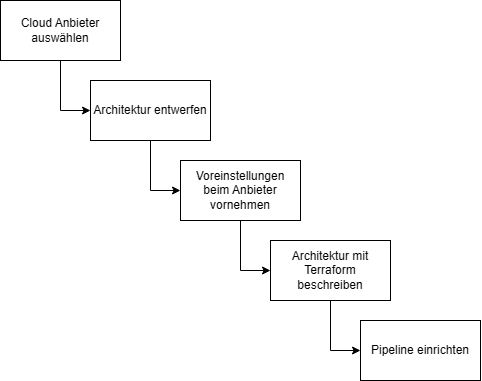
\includegraphics[width=0.76\textwidth]{../Phase2/pics/Vorgehensweise.png}
\caption{Vorgehensmodell aus Phase 2 als Basis für die Endphase}
\end{figure}

Die praktische Umsetzung war dabei bewusst als Schleife organisiert und nicht als einmaliger ``Big-Bang''-Deploy. Nach jedem technischen Schritt wurde geprüft, ob das Ergebnis noch zur Zielsetzung passt: Nach Infrastrukturänderungen folgte \texttt{terraform validate}, bei Containeränderungen ein erneuter Build/Push-Zyklus, und bei Routing-Anpassungen eine Erreichbarkeits- und Failover-Prüfung über den Front-Door-Endpunkt. Dieser zyklische Ansatz hat zwei Vorteile gebracht: Fehler wurden früh erkannt, und die Auswirkung einzelner Änderungen blieb klar nachvollziehbar.

\subsection{Explizite Entscheidungskriterien}
Die Auswahl der Cloud-Dienste erfolgte explizit entlang messbarer Kriterien:

\begin{itemize}
  \item \textbf{Hohe Verfügbarkeit}: aktive Bereitstellung in mindestens zwei Regionen.
  \item \textbf{Automatische Skalierung}: native Lastskalierung ohne manuelles Node-Management.
  \item \textbf{Sicherheit}: TLS-Absicherung, least-privilege Zugriff und Härtung von HTTP-Responses.
  \item \textbf{Betriebsaufwand}: möglichst geringer Plattform-Overhead (managed Services statt Self-Managed Cluster).
  \item \textbf{Automatisierbarkeit}: IaC- und CI/CD-Fähigkeit mit stabilen Providern und klaren APIs.
  \item \textbf{Kosten- und Komplexitätsprofil}: angemessen für einen kleinen, aber realistischen Demonstrator.
\end{itemize}

\subsection{Plattformvergleich und kritische Beurteilung}
Fachlich wären mehrere Plattformkombinationen möglich gewesen. Die Entscheidung wurde nicht über ein einzelnes Kriterium getroffen, sondern als Trade-off:

\begin{table}[H]
\centering
\caption{Vergleich möglicher Plattformoptionen}
\begin{tabular}{p{0.20\textwidth}p{0.23\textwidth}p{0.23\textwidth}p{0.23\textwidth}}
\toprule
\textbf{Kriterium} & \textbf{Azure (gewählt)} & \textbf{AWS (Alternative)} & \textbf{GCP (Alternative)} \\
\midrule
Globales Routing & Front Door mit Anycast, Health Probe und Failover & CloudFront + Route 53 + ALB & Cloud CDN + Global LB \\
Containerbetrieb & Container Apps (serverless, autoscaling) & ECS/Fargate oder EKS & Cloud Run oder GKE \\
IaC-Reife & Terraform AzureRM gut etabliert & Terraform AWS sehr ausgereift & Terraform Google ausgereift \\
Betriebsaufwand & gering bis mittel (managed) & mittel (je nach ECS/EKS Wahl) & gering bis mittel \\
Projektfit & sehr gut: direkte Kombination Front Door + ACA & gut, aber mehr Integrationsaufwand im Entwurf & gut, aber geringere Vorerfahrung im Team \\
\bottomrule
\end{tabular}
\end{table}

\textbf{Kritische Bewertung:}
Die Wahl von Azure ist für diese Problemstellung sinnvoll, weil Front Door und Container Apps die Kernanforderungen direkt adressieren. Die Alternative \textit{AKS + Ingress + eigener globaler Traffic-Manager} wäre flexibler, hätte jedoch den Betriebsaufwand unverhältnismäßig erhöht. Ebenfalls möglich wäre eine \textit{Static-Web-App-Lösung} gewesen; diese wäre für reinen HTML-Content einfacher, bietet aber weniger Lernwert für containerisierte Multi-Region-Deployments und spätere Backend-Erweiterungen.

\subsection{Cloud-Architektur als Zielbild}
Das frühe Architekturziel aus Phase 1 wurde in Phase 2/3 konkretisiert. Die folgenden Diagramme zeigen die Entwicklung vom Konzept zur umgesetzten Struktur:

\begin{figure}[H]
\centering
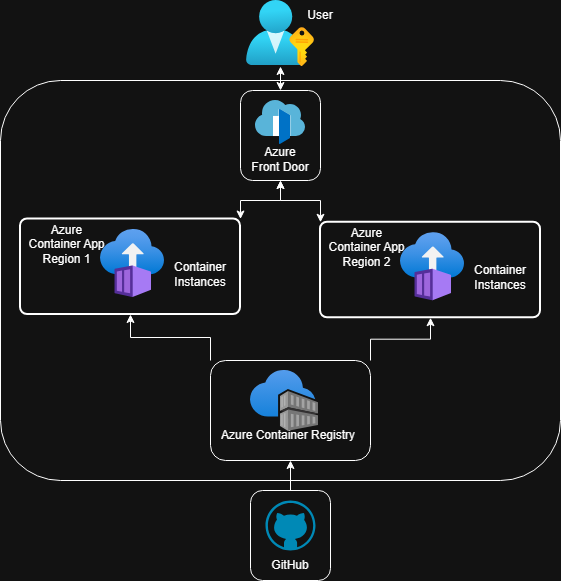
\includegraphics[width=0.5\textwidth]{../Phase2/pics/CloudArchitecture.Compact.png}
\caption{Kompakte Umsetzungsarchitekture}
\end{figure}

\section{Lösung: Technische Umsetzung und IaC-Struktur}
\subsection{Architektur der implementierten Lösung}
Die finale Lösung besteht aus folgenden Schichten:

\begin{enumerate}
  \item \textbf{Artefakt-Schicht}: Docker-Image der statischen Web-App.
  \item \textbf{Registry-Schicht}: Azure Container Registry (ACR) für Image-Hosting.
  \item \textbf{Compute-Schicht}: zwei Azure Container Apps (Primary/Secondary) in verschiedenen Regionen.
  \item \textbf{Observability-Schicht}: je Region ein Log-Analytics-Workspace und ein Container-App-Environment.
  \item \textbf{Edge-Schicht}: Azure Front Door als globaler Einstiegspunkt mit HTTPS-Weiterleitung und Health-basiertem Routing.
  \item \textbf{Identity-Schicht}: User Assigned Managed Identity und \texttt{AcrPull}-Rolle für Registry-Zugriffe.
\end{enumerate}

Der Request-Fluss ist klar definiert: Client $\rightarrow$ Front Door Endpoint $\rightarrow$ gesundes Origin (primär, ansonsten sekundär) $\rightarrow$ Container App Ingress.

\subsection{IaC-Struktur über ``Module'' und Variablen}
Auch ohne ausgelagerte Terraform-Unterordner ist die Infrastruktur fachlich modular organisiert. Die Dateigruppierung im Ordner \texttt{infra/} bildet logische Module:

\begin{table}[H]
\centering
\caption{Logische Terraform-Module nach Verantwortungsbereich}
\begin{tabular}{p{0.28\textwidth}p{0.32\textwidth}p{0.30\textwidth}}
\toprule
\textbf{Bereich} & \textbf{Dateien} & \textbf{Aufgabe} \\
\midrule
Core & \texttt{versions.tf}, \texttt{resource-group.tf}, \texttt{locals.tf}, \texttt{variables.tf} & Provider, Backend, Grundparameter, Namenslogik \\
Registry + Identity & \texttt{acr.tf}, \texttt{identity.tf} & ACR-Erstellung/Nutzung, Rollenrechte für Pull \\
Runtime & \texttt{log-analytics.tf}, \texttt{container-app-envs.tf}, \texttt{container-apps.tf} & Laufzeitumgebung und Workload in zwei Regionen \\
Edge & \texttt{frontdoor.tf} & Globales Routing, Health Probe, HTTPS-Policy \\
Outputs & \texttt{outputs.tf} & Ausgabe von Endpunkten und zentralen IDs \\
\bottomrule
\end{tabular}
\end{table}

Die Variablen in \texttt{variables.tf} steuern den Betriebsmodus (z.\,B. bestehende ACR nutzen oder neue ACR anlegen), den Image-Stand, Regionen sowie Skalierungsgrenzen. Damit bleibt die Lösung reproduzierbar, aber gleichzeitig konfigurierbar.

\subsection{Detaillierter Ablauf von der Änderung bis zum laufenden Dienst}
Der technische Ablauf ist nicht nur ``Skript starten und warten'', sondern besteht aus mehreren kontrollierten Zustandsübergängen. Diese Trennung ist wichtig, weil Anwendungsartefakte (Docker-Image) und Infrastrukturzustand (Terraform-State) unterschiedliche Lebenszyklen haben.

\textbf{Phase 1: Änderung und lokaler Vorab-Check.}
Am Anfang steht eine inhaltliche Änderung im Repository, z.\,B. an \texttt{app/index.html}, \texttt{nginx.conf} oder \texttt{infra/*.tf}. Vor dem eigentlichen Rollout wird geprüft, ob die Änderung syntaktisch und logisch sauber ist. Für die Infrastruktur heißt das konkret: erst \texttt{terraform fmt} und \texttt{terraform validate}, danach erst \texttt{plan/apply}. So werden vermeidbare Fehler (wie in Phase 3 beim Variablen-Validierungsproblem) bereits vor dem produktiven Schritt abgefangen.

\textbf{Phase 2: Secrets- und Kontextauflösung.}
Das Deployment-Skript liest die benötigten Parameter aus Azure Key Vault (z.\,B. Registry-Name, State-Storage, Service-Principal-Daten). Dadurch liegen betriebsrelevante Werte nicht hart im Code. Gleichzeitig wird ein klarer Laufkontext erzeugt: Subscription, Ziel-Regionen, Image-Tag und State-Key sind für diesen Lauf eindeutig gesetzt.

\textbf{Phase 3: Build- und Artefaktfluss.}
Das Docker-Image wird lokal gebaut und mit konsistenter Tag-Strategie in ACR abgelegt. Erst wenn der Push erfolgreich ist, folgt der Infrastrukturteil. Damit ist sichergestellt, dass Terraform nicht auf ein nicht vorhandenes oder veraltetes Artefakt zeigt. Dieser Schritt reduziert ``halbfertige'' Deployments, bei denen Infrastruktur schon aktualisiert wurde, aber das neue Image noch fehlt.

\textbf{Phase 4: Terraform-Initialisierung und geordnete Bereitstellung.}
Nach dem Build wird das Remote-Backend initialisiert und anschließend in zwei Stufen ausgerollt: zuerst ein gezielter Bootstrap für die Grundressourcen, danach das vollständige \texttt{apply}. Diese Reihenfolge verbessert die Fehlersuche, weil Abhängigkeiten (Resource Group, Registry-Kontext, Identity) bereits stabil stehen, bevor globale Komponenten wie Front Door final verdrahtet werden.

\textbf{Phase 5: Aktivierung im Datenpfad.}
Sobald beide Container Apps laufen, bedient Front Door den globalen Einstieg. Health-Probes steuern, welches Origin aktiv priorisiert wird. Das bedeutet: Bei stabiler Primärregion fließt Traffic wie geplant dorthin; bei Störung übernimmt die Sekundärregion, ohne dass der öffentliche Endpunkt geändert werden muss.

\textbf{Phase 6: Nachkontrolle und Betriebsroutine.}
Nach dem Rollout werden Endpunkte und Outputs geprüft (\texttt{frontdoor\_url}, primäre/sekundäre FQDNs). Für den Regelbetrieb bedeutet das: Änderungen werden klein gehalten, reproduzierbar eingespielt und jeweils mit einer kurzen technischen Verifikation abgeschlossen. Genau diese Routine trennt ein einmaliges Demo-Deployment von einem belastbaren Betriebsprozess.

\subsection{Reproduzierbare Deployment-Schritte}
\textbf{Voraussetzungen}
\begin{itemize}
  \item Azure CLI, Docker und Terraform lokal installiert.
  \item Zugriff auf Azure Subscription und auf ein Key Vault mit den benötigten Secrets.
  \item Repo im lokalen Dateisystem ausgecheckt.
\end{itemize}

\textbf{Minimaler Ablauf über das Projektskript}
\begin{enumerate}
  \item \texttt{KEYVAULT\_NAME} setzen (optional \texttt{KEYVAULT\_SUBSCRIPTION\_ID}).
  \item Im Projektroot \texttt{scripts\textbackslash terraform-local.cmd} ausführen.
  \item Das Skript liest Secrets, loggt den Service Principal ein, baut/pusht das Image und startet \texttt{terraform init/apply}.
  \item Ergebnisprüfung über Terraform-Outputs (\texttt{frontdoor\_url}, \texttt{container\_app\_*\_fqdn}).
\end{enumerate}

Für eine kontrollierte Ausführung empfiehlt sich zusätzlich ein expliziter Prüfpfad im \texttt{infra}-Ordner, bevor produktive Änderungen übernommen werden. Damit wird der Ablauf transparenter und besser dokumentierbar, insbesondere bei Teamarbeit oder bei Änderungen an sicherheitsrelevanten Ressourcen.

\begin{lstlisting}[language=bash,caption={Empfohlener IaC-Prüfpfad vor produktivem Apply}]
cd infra
terraform fmt -check
terraform validate
terraform plan -out=tfplan
terraform apply tfplan
\end{lstlisting}

Der Vorteil dieser Reihenfolge liegt in der Trennung von \textit{Prüfen} und \textit{Ausführen}: Das geplante Ergebnis wird sichtbar, bevor echte Änderungen geschrieben werden. Gerade bei Front-Door-Routen, Rollenzuweisungen oder Skalierungsgrenzen verringert das das Risiko ungewollter Seiteneffekte.

\textbf{Wichtige technische Schritte im Detail}
\begin{lstlisting}[language=bash,caption={Konzeptioneller Deployment-Ablauf}]
az login
set KEYVAULT_NAME=<name>
scripts\terraform-local.cmd

# intern im Skript:
# 1) Key Vault Secrets lesen
# 2) Docker Image bauen und nach ACR pushen
# 3) Terraform Backend initialisieren
# 4) Terraform Apply in Multi-Region-Architektur
\end{lstlisting}

Die Pipeline-Logik aus Phase 2 bleibt als Referenz für den automatisierten Build-/Push-Pfad erhalten:


\begin{figure}[H]
\centering
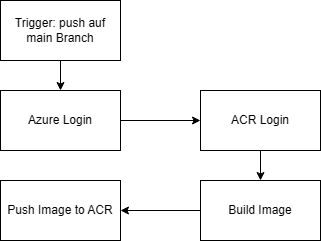
\includegraphics[width=0.76\textwidth]{../Phase2/pics/PipelineAblauf.png}
\caption{Pipelineablauf als reproduzierbares Liefermuster}
\end{figure}

\subsection{Best Practices in der Umsetzung}
Die Implementierung folgt mehreren bewährten Mustern:

\begin{itemize}
  \item \textbf{Least Privilege}: Zugriff auf ACR über Managed Identity + \texttt{AcrPull} statt statischer Credentials.
  \item \textbf{Parametrisierung}: Regionen, Image, Skalierung und Endpunktnamen über Variablen steuerbar.
  \item \textbf{Health-basiertes Routing}: Front Door prüft Origin-Gesundheit und priorisiert das primäre Ziel.
  \item \textbf{State-Konsistenz}: Remote State im Azure Storage für reproduzierbare Teamabläufe.
  \item \textbf{Sicherheits-Hardening}: HTTPS-Weiterleitung plus Header-Hardening auf NGINX-Ebene.
\end{itemize}

Zusätzlich zeigt der aktuelle Stand, dass Stabilität nicht nur aus ``richtigen'' Ressourcen entsteht, sondern aus sauberer Reihenfolge und klarer Verantwortlichkeit: Artifact-Pfad, Infrastruktur-Pfad und Edge-Konfiguration sind getrennt dokumentiert. Das erleichtert Wartung, weil bei einem Fehler schneller erkennbar ist, ob Ursache und Lösung eher im Container, in Terraform oder im globalen Routing liegen.

\section{In Phase 3 gelöste Issues}
\subsection{Issue 1: Terraform-Validierungsfehler in \texttt{variables.tf}}
\textbf{Problemstellung:} In einer früheren Version wurde im \texttt{validation}-Block der Variable \texttt{acr\_name} auf eine andere Variable (\texttt{var.use\_existing\_acr}) referenziert. Terraform-Validierungen dürfen jedoch nur den Wert der \emph{selben} Variable auswerten.

\textbf{Auswirkung:} \texttt{terraform validate} schlug fehl; damit war ein sauberer Deploy-Prozess blockiert.

\textbf{Ursache:} Falsches Validierungsmuster in der Variablendefinition.

\textbf{Lösung in Phase 3:}
\begin{itemize}
  \item Entfernen der abhängigen Validierung, die fremde Variablen referenziert.
  \item Beibehaltung einer gültigen, lokalen Validierung nur für \texttt{var.acr\_name} (Regex für 5--50 Zeichen, lowercase alphanumerisch).
\end{itemize}

\begin{lstlisting}[caption={Gültiges Validierungsmuster für acr\_name in der aktuellen Struktur}]
variable "acr_name" {
  type        = string
  description = "Optional ACR name override (lowercase alphanumeric, 5-50 chars)."
  default     = null

  validation {
    condition     = var.acr_name == null || can(regex("^[a-z0-9]{5,50}$", var.acr_name))
    error_message = "If provided, acr_name must be 5-50 lowercase letters/numbers only."
  }
}
\end{lstlisting}

\textbf{Ergebnis:} Die Validierungsphase ist wieder stabil; die Infrastruktur kann ohne diese Blockade ausgerollt werden.

\subsection{Issue 2: HTTPS erzwungen, aber fehlende Security Header}
\textbf{Problemstellung:} Front Door erzwingt HTTPS bereits korrekt, jedoch fehlten in einer früheren NGINX-Konfiguration zusätzliche Header wie CSP oder HSTS.

\textbf{Risiko:} Erhöhtes Angriffsfenster für XSS, Clickjacking und schwache Browser-Sicherheitsrichtlinien.

\textbf{Lösung in Phase 3:}
\begin{itemize}
  \item Nutzung einer expliziten \texttt{nginx.conf} statt nur Standard-NGINX-Defaults.
  \item Ergänzung sicherheitsrelevanter Header mit \texttt{add\_header ... always}.
\end{itemize}

\begin{table}[H]
\centering
\caption{Sicherheitsheader und ihr Beitrag}
\begin{tabular}{p{0.36\textwidth}p{0.54\textwidth}}
\toprule
\textbf{Header} & \textbf{Nutzen} \\
\midrule
\texttt{Content-Security-Policy} & Schränkt erlaubte Quellen ein und reduziert XSS-Risiken \\
\texttt{Strict-Transport-Security} & Erzwingt HTTPS im Browser (HSTS) \\
\texttt{X-Frame-Options} & Schutz gegen Clickjacking \\
\texttt{X-Content-Type-Options} & Verhindert MIME-Type-Sniffing \\
\texttt{Referrer-Policy} & Kontrolliert Weitergabe von Referrer-Informationen \\
\texttt{Permissions-Policy} & Schaltet sensible Browser-Features gezielt ab \\
\bottomrule
\end{tabular}
\end{table}

\textbf{Ergebnis:} Die Transportverschlüsselung durch Front Door wird jetzt um browserseitige Sicherheitskontrollen in der Anwendungsschicht ergänzt. Dadurch steigt die technische Reife der Lösung deutlich.

\section{Lessons Learned}
\subsection{Technische Erkenntnisse}
\begin{enumerate}
  \item \textbf{IaC-Validierung früh einplanen:} Kleine Verstöße gegen Terraform-Regeln (wie variable-übergreifende Validation) blockieren komplette Deployments.
  \item \textbf{HTTPS allein reicht nicht:} Security Header sind ein notwendiger zweiter Schutzring auf Anwendungsebene.
  \item \textbf{Logische Modularisierung hilft:} Auch ohne echte Terraform-Unterordner erhöht eine klare Dateistruktur die Wartbarkeit.
  \item \textbf{Identity-first Design reduziert Risiken:} Managed Identities und Rollen sind robuster als statische Zugangsdaten.
  \item \textbf{Automatisierung ist ein Qualitätsmerkmal:} Wiederholbare Skripte und klarer State reduzieren Fehler bei manuellen Eingriffen.
\end{enumerate}

\subsection{Organisatorische und methodische Erkenntnisse}
\begin{itemize}
  \item Entscheidungskriterien sollten früh schriftlich fixiert werden; spätere Architekturdebatten werden dadurch kürzer und sachlicher.
  \item Diagramme über mehrere Phasen hinweg weiterzuentwickeln verbessert Teamkommunikation und Nachvollziehbarkeit.
  \item Issues sollten nicht nur gefixt, sondern mit Ursache, Auswirkung und Verifikation dokumentiert werden.
\end{itemize}

\section{Zusammenfassung und Zukunftsblick}
Die Projektidee wurde von der Anforderungsanalyse bis zur produktionsnahen Cloud-Lösung konsistent umgesetzt. Die gewählte Architektur adressiert Verfügbarkeit, globale Erreichbarkeit, Skalierbarkeit und Sicherheit mit einem vertretbaren Betriebsaufwand. Durch Terraform ist die Infrastruktur reproduzierbar, und durch die in Phase 3 gelösten Issues wurde die technische Qualität weiter stabilisiert.

Für den nächsten Reifegrad sind insbesondere folgende Erweiterungen sinnvoll:
\begin{enumerate}
  \item \textbf{Messbare Last- und Failover-Tests} zur quantitativen Absicherung der nicht-funktionalen Ziele.
  \item \textbf{Private Netzgrenzen für kritische Dienste.} Der nächste sinnvolle Schritt ist, ACR und weitere sensible Komponenten nicht mehr standardmäßig öffentlich erreichbar zu lassen, sondern über Private Endpoints und VNet-Integration zu führen. In Kombination mit Subnetzen für die Container-App-Umgebungen würde der Datenpfad stärker innerhalb des Azure-Netzes bleiben.
  \item \textbf{Gezielte Netzwerksteuerung über NSGs.} Ergänzend zur VNet-Integration sollten Network Security Groups explizit eingehende und ausgehende Regeln steuern. Damit wird Netzwerkzugriff nicht implizit über Defaults, sondern explizit über dokumentierte Sicherheitsregeln freigegeben.
  \item \textbf{IAM-Governance über reine ACR-Rechte hinaus.} Die aktuelle Identity-Nutzung ist für den Image-Pull gut umgesetzt. Als Ausbaupfad bietet sich ein regelmäßiges Rollen-Audit für weitere Ressourcen (z.\,B. Monitoring, Edge-Komponenten, zukünftiger Key Vault) an, damit Berechtigungen dauerhaft minimal bleiben.
  \item \textbf{Secrets-Management vollständig in die Infrastruktur integrieren.} Obwohl das lokale Skript bereits auf Key-Vault-Werte zugreift, fehlt noch ein vollständig per Terraform bereitgestellter Key Vault mit klaren Zugriffsrichtlinien über Managed Identities. Das vereinfacht Rotation und reduziert verteilte Secret-Ablagen.
  \item \textbf{CI/CD als technische Qualitätsbarriere ausbauen.} Nach dem Image-Push sollten in der Pipeline standardmäßig \texttt{terraform validate}, \texttt{plan} und erst danach ein kontrolliertes \texttt{apply} folgen. Ergänzend sind automatisierte Checks wie \texttt{tflint}, Security-Scans (z.\,B. IaC-Scan und Container-Scan) und ein separates Deployment je Zielumgebung sinnvoll.
  \item \textbf{Operative Überwachung von ``beobachten'' auf ``reagieren'' heben.} Der aktuelle Stand sammelt Logs, aber der nächste Schritt sind konkrete Alert-Regeln für Fehlerquoten, CPU/Memory und Verfügbarkeitsindikatoren sowie Budget- und Kostenalarme. So wird Monitoring vom passiven Dashboard zum aktiven Betriebswerkzeug.
\end{enumerate}

Damit entsteht ein belastbarer Weg von einem Lernprojekt zu einer robusteren, produktionsnahen Zielarchitektur.

\end{document}
